\chapter{Intensity measurements}

In the previous chapter we seeked for different aspects of the \gls{rf}
signal powering the \gls{aod} elements. Down the road we had to realize that
there are many forces at work which at large are difficult to account for.
That in mind we proceed with the analysis of the deflected laser beam
intensity subject to the configured frequency and relative amplitude of the
synthesized output \gls{rf} output signal.

\section{Intensity control}

The laser intensity is regulated by a control loop with \gls{aom} in order to
intercept power drifts from the laser source. This control loop is tightly
integrated into our experimental setup and thus will be present for all
subsequent intensity measurements. In this section we want to discuss the
grade of this control loop and estimate its error contribution.

\subsection{Setup}

\begin{figure}[h]
  \centering
  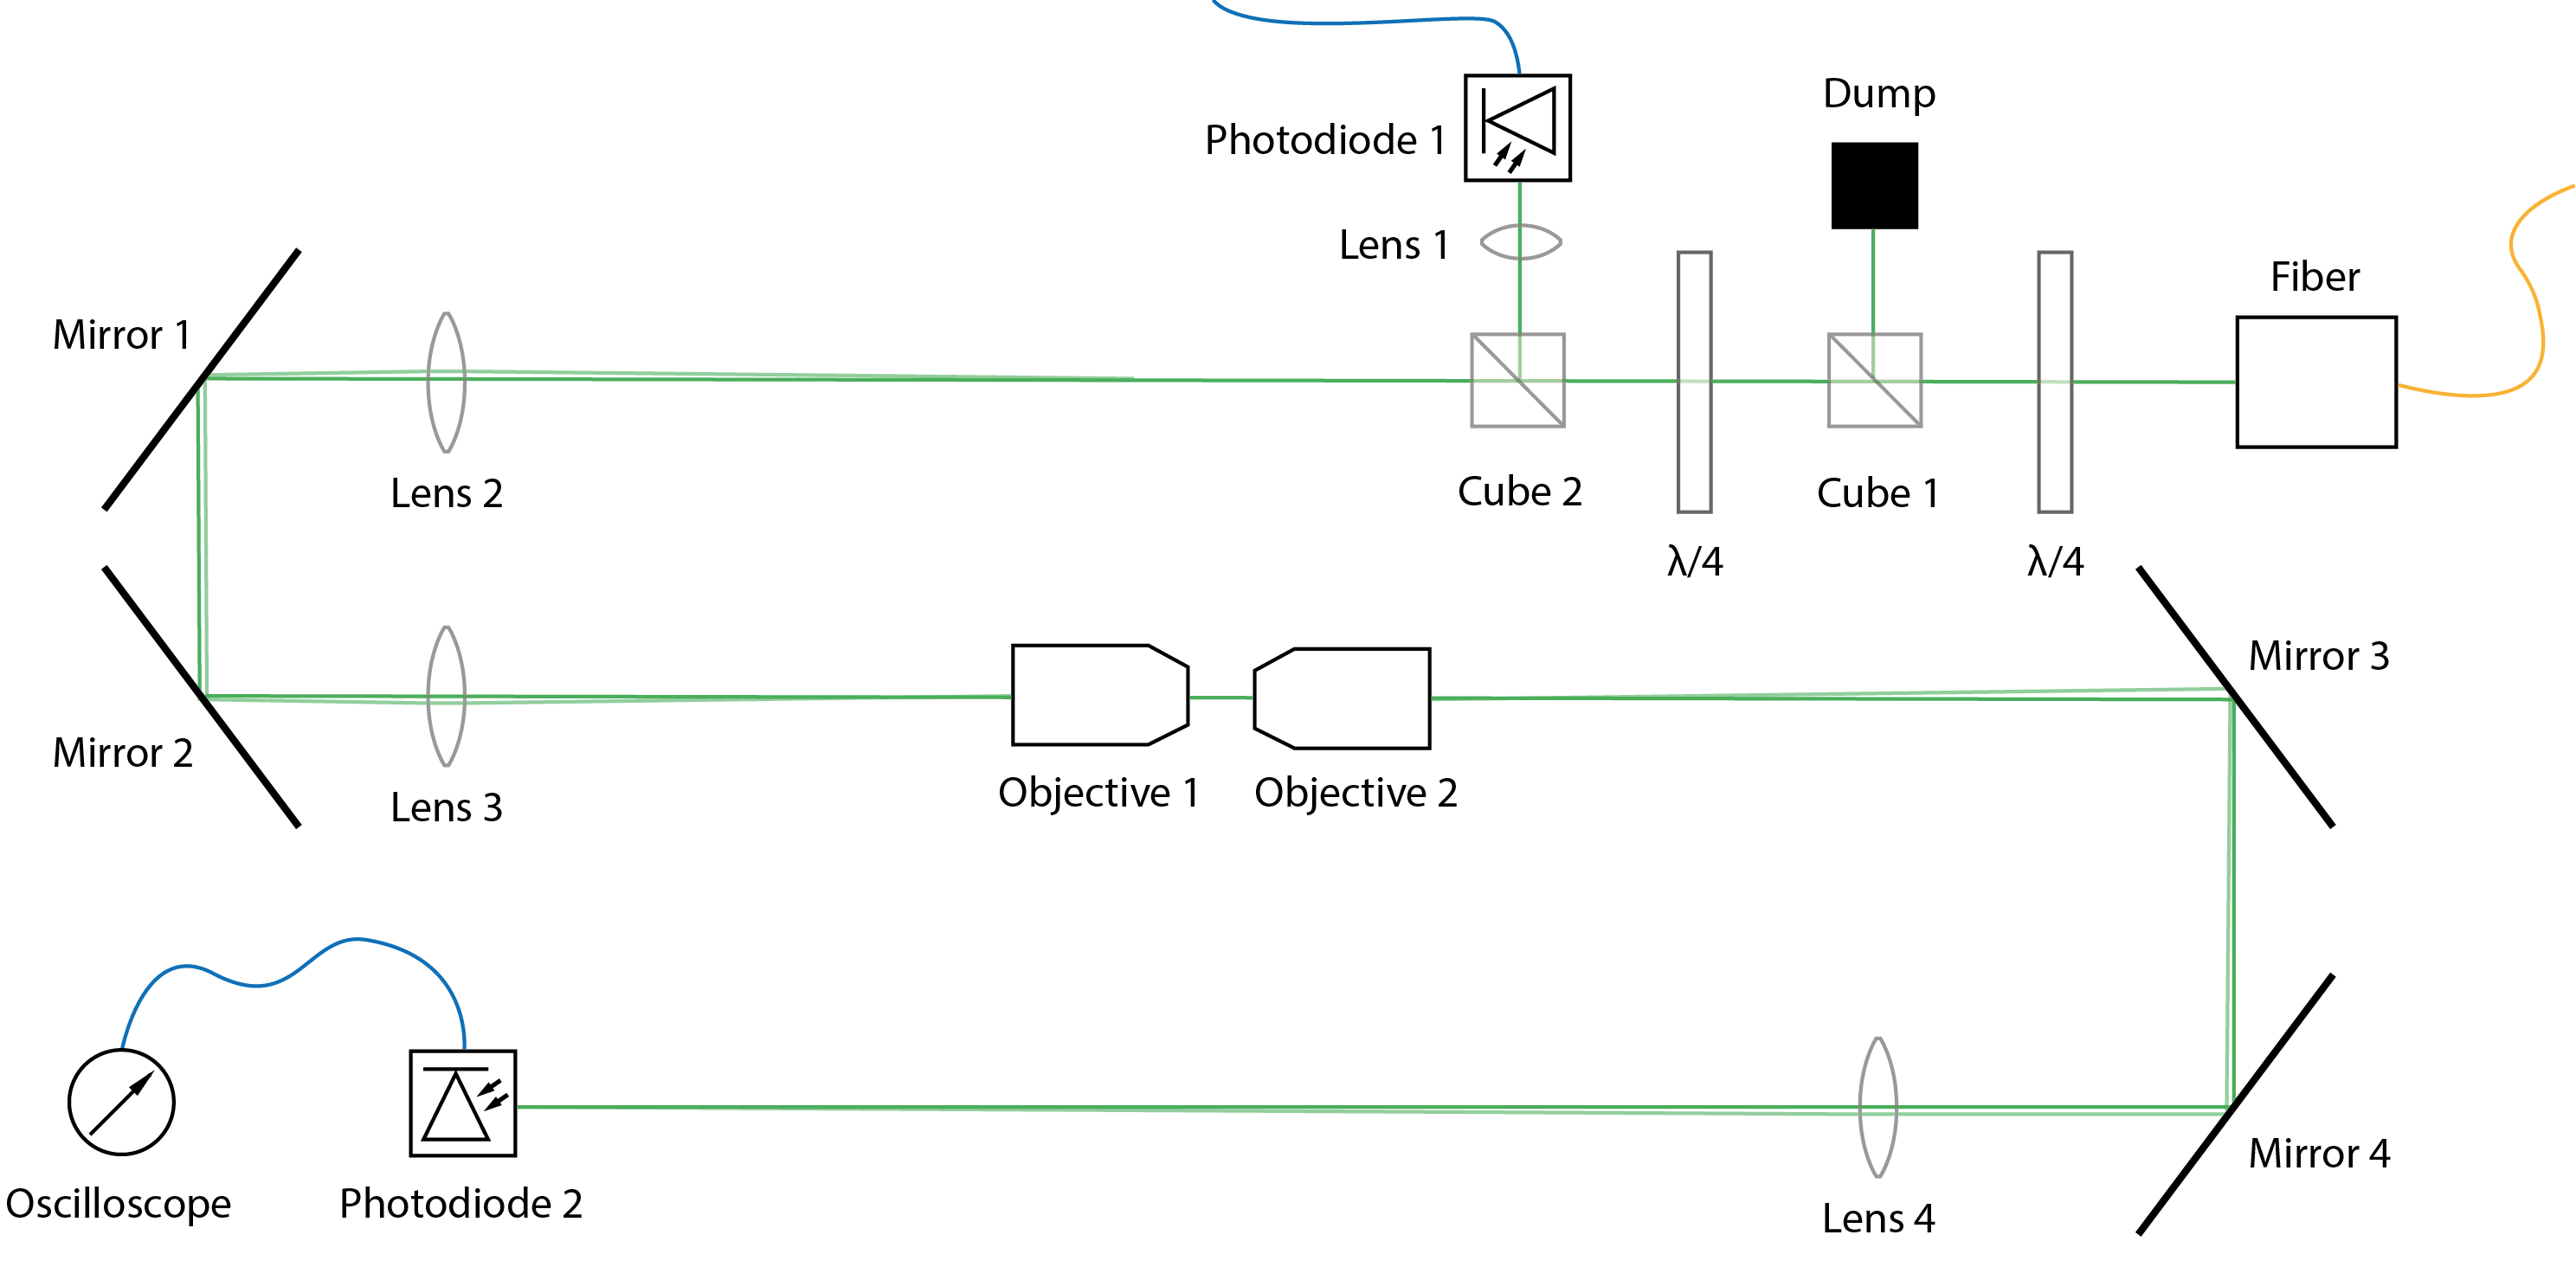
\includegraphics[width=\textwidth]{\mediadir{setup/intensity-control.png}}
  \captionsetup{width=.8\textwidth}
  \caption{Optical and electronic setup of the intensity control experiment.
  The \gls{aod}s have been removed. The beam hits photodiode 2 that is
connected to the oscilloscope.}
  \label{fig:intensity_control_setup}
\end{figure}

The experimental setup is the same as described in XX but with disassembled
\gls{aod} and photodiode 2 as the terminus of the laser beam. The setup is
depicted in \Cref{fig:intensity_control_setup}. The photodiode gain was set
to \SI{50}{\decibel}.

\subsection{Long term measurement}

In the long term measurement we were interested in the long term behaviour
of the intensity control loop. In particular if there are oscillations or
intensity collapses.

Therefore we obtained voltage measurements in an interval of about
\SI{2}{\minute} over a total time of approximately \SI{16}{\hour}.

\begin{figure}[ht]
  \centering
  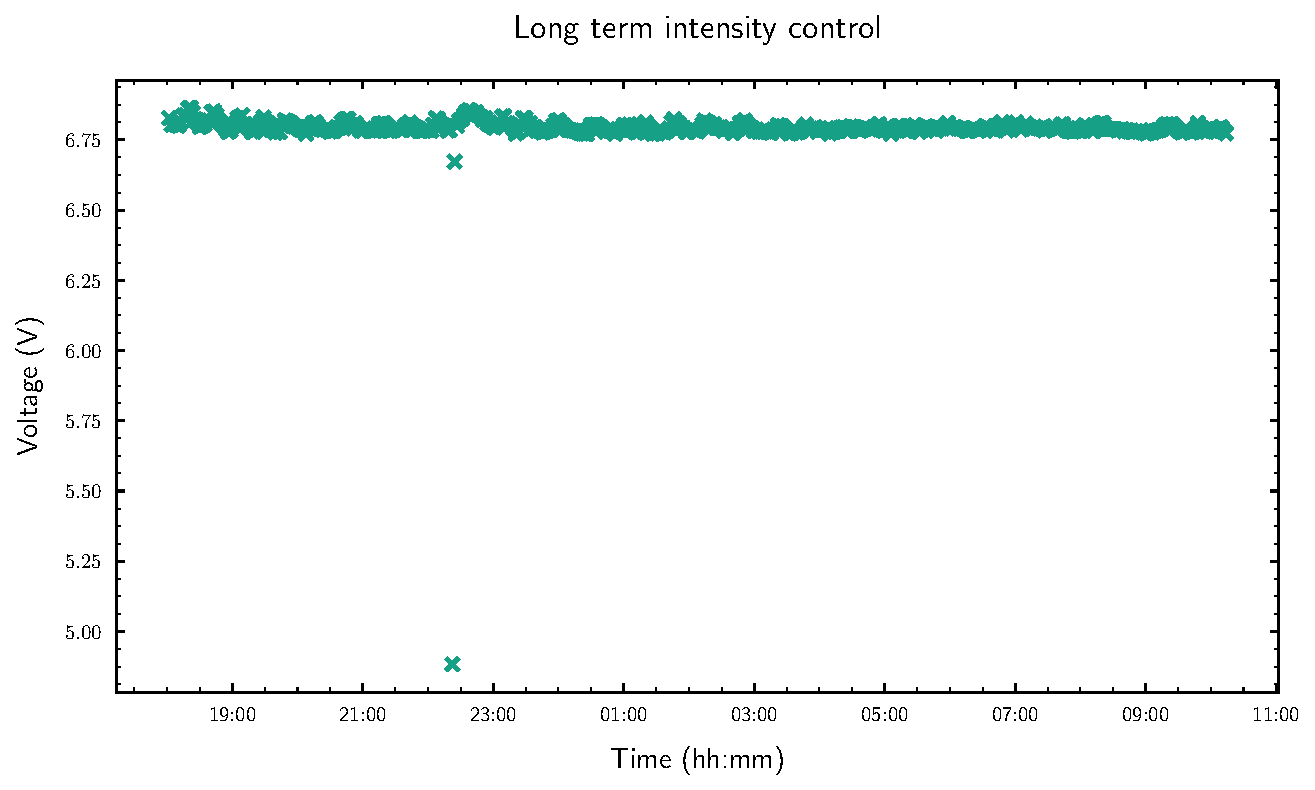
\includegraphics[width=\textwidth]{\figuredir{intensity/control/long.pdf}}
  \captionsetup{width=.8\textwidth}
  \caption{Long term measurement of the intensity with controlled intensity.
    The intensity was measured every \SI{2}{\minute} for over \SI{16}{\hour}
    to determine the accuracy of the intensity controller. The outlier at
    about 22:45 was caused by laboratory visit otherwise the intensity remains
  stable.}
  \label{fig:intensity_control_long}
\end{figure}

The voltage time series is shown in \Cref{fig:intensity_control_long}. We 
note outliers at about 22:45 which were probably caused by a late laboratory
visit. Further we see a constant albeit noisy intensity signal. In comparison
we could watch real time oscillations and drifts when disabling the control
loop.

\Cref{tab:intensity_control_long} depicts the descriptive statistics belonging
to the voltage time series visualized in \Cref{fig:intensity_control_long}.
The mean intensity is measured to be around \SI{6.79}{\volt} with peaks up
to \SI{6.86}{\volt}. The standard deviation yields us a relative error of
around \SI{1.4}{\percent}.

\begin{table}[h]
  \centering
  \begin{tabular}{|c|c|c|c|}
    \hline
    Mean & Minimum & Maximum & Standard deviation \\
    \hline
    \SI{6.79}{\volt} &
    \SI{4.88}{\volt} &
    \SI{6.86}{\volt} &
    \SI{0.09}{\volt} \\
    \hline
  \end{tabular}
  \captionsetup{width=.8\textwidth}
  \caption{Descriptive statistics of the short term measurement of the
  intensity with controlled intensity. Note the small standard deviation.}
  \label{tab:intensity_control_long}
\end{table}

\subsection{Short term measurement}

The previous section gave us already some good insights about the long term
stability of the intensity control loop. Yet in practice typical intensity
measurements are of much smaller magnitude, henceforth it seems close at hand
to also conduct a short term measurement.

\begin{table}[h]
  \centering
  \begin{tabular}{|c|c|c|c|}
    \hline
    Mean & Minimum & Maximum & Standard deviation \\
    \hline
    \SI{6.78}{\volt} &
    \SI{6.77}{\volt} &
    \SI{6.82}{\volt} &
    \SI{0.01}{\volt} \\
    \hline
  \end{tabular}
  \captionsetup{width=.7\textwidth}
  \caption{Descriptive statistics of the short term measurement of the
  intensity with controlled intensity. Note the small standard deviation.}
  \label{tab:intensity_control_short}
\end{table}

For the short term measurement time parameters were adjusted to a sample
interval of \SI{10}{\second} and measurment were performed over \SI{1}{\hour}.

\begin{figure}[ht]
  \centering
  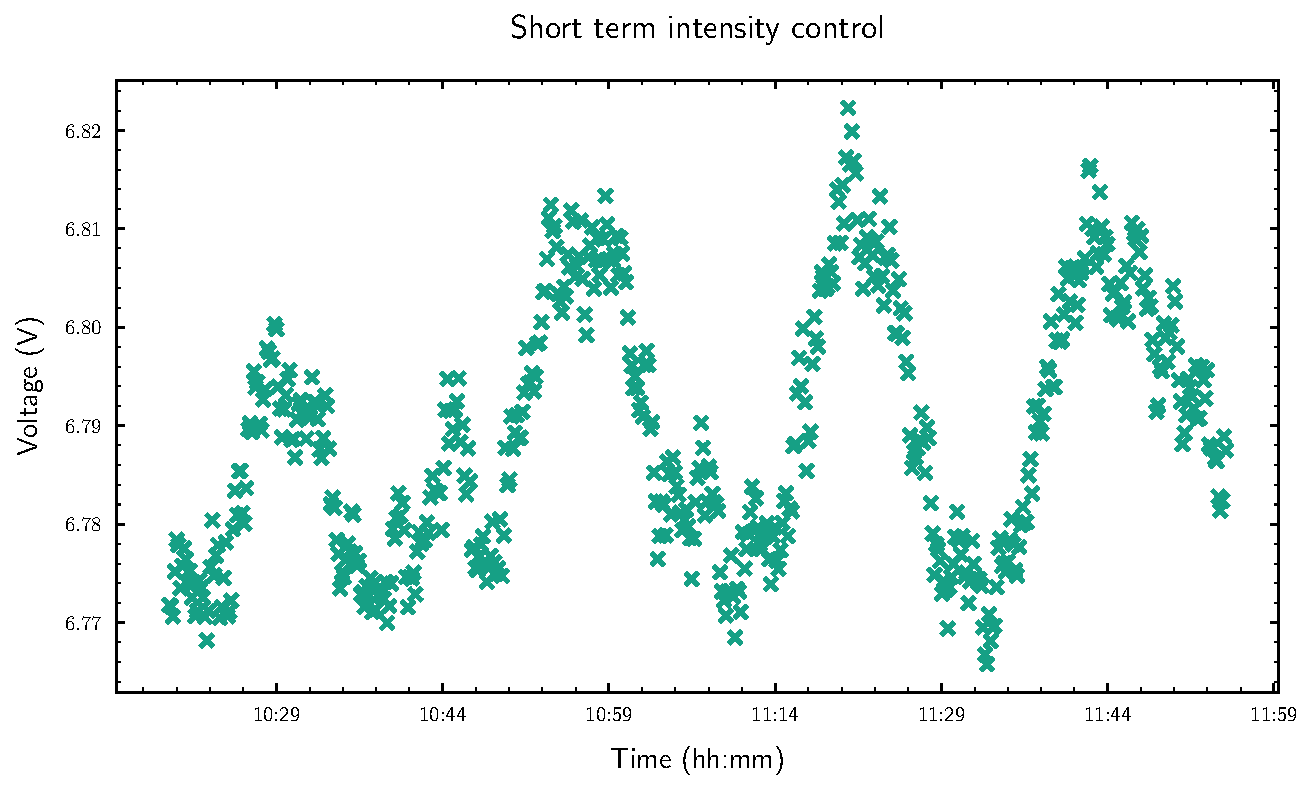
\includegraphics[width=\textwidth]{\figuredir{intensity/control/short.pdf}}
  \captionsetup{width=.8\textwidth}
  \caption{Short term measurement of the intensity with controlled intensity.
    The intensity was measured every \SI{10}{\second} for over \SI{1}{\hour}
    to determine the accuracy of the intensity controller.}
  \label{fig:intensity_control_short}
\end{figure}

The intensity time series of the short term measurement is depicted in
\Cref{fig:intensity_control_short} and the associated descriptive
statistics are presented in \Cref{tab:intensity_control_short}.

On a smaller timescale we see that the intensity control loop performs
periodic oscillations, however the descriptive statistics show much smaller
deviation from the mean, than observed in the long term measurements. As we
do not see outliers in \Cref{fig:intensity_control_short} we can pay more
attention to the value range of \SI{0.05}{\volt} which was obfuscated in
the long term measurement because of outliers.

\subsection{Summary}

The previous discussion confirmed that the intensity is regulated in that
we only observe oscillations around the targeted intensity value. Yet we are
still missing statements with regard to the magnitude of these oscillations
as we are missing a comparison to real intensity data.

\begin{table}[ht]
  \centering
  \begin{tabular}{|c|c|c|}
    \hline
    Measurement & Value range & Standard deviation \\
    \hline
    long term & \SI{1.98}{\volt} & \SI{0.09}{\volt} \\
    \hline
    short term & \SI{0.06}{\volt} & \SI{0.01}{\volt} \\
    \hline
    typical & \SI{1.43}{\volt} & \SI{0.40}{\volt} \\
    \hline
  \end{tabular}
  \captionsetup{width=.8\textwidth}
  \caption{Descriptive statistics of the short and long term measurement
  of the intensity control and a typical intensity measurements where we
subtracted the mean intensity for comparison.}
  \label{tab:intensity_control}
\end{table}

For a typical measurement, to compare the intensity oscillations with, we
elected the intensity progression of a linear frequency sweep of the
\gls{aod} in the vertical socket while the \gls{aod} in the horizontal socket
is fixed. We will discuss this specific meausurement in detail in a later
section. In \Cref{tab:intensity_control} we see some statistics of the
long and short term measurements next to the typical measurement.

\begin{figure}[ht]
  \centering
  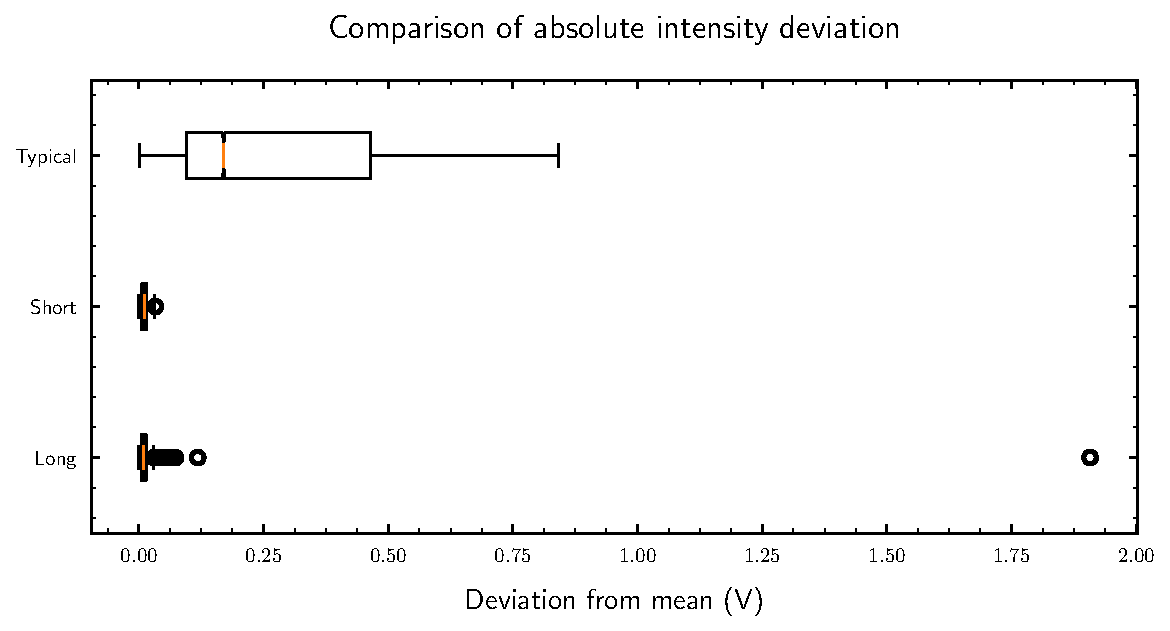
\includegraphics[width=\textwidth]{\figuredir{intensity/control/deviation.pdf}}
  \captionsetup{width=.8\textwidth}
  \caption{Boxplot of the long and short term intensity measurements and a typical
  intensity measurement with the \gls{aod} where we subtracted the mean intensity
  for comparison. The typical measurements covers a much wider intensity range
then deviations from the intensity control loop.}
  \label{fig:intensity_control_comparison}
\end{figure}

One dismally error estimate would be the quotient of the value range of the
short term measurement and the typical measurement, yielding an error of
\SI{4.2}{\percent}. A second approach would be the quotient of the standard
deviation of the short term and typical measurement, yielding
\SI{2.5}{\percent} error. When comparing the typical measurement to the
statictis of a long term measurement we find rather large errors which
suggests that there re other statistical key figures which may be more
suitable.

A boxplot is very useful in visualizing the spread. We have an orange stripe
marking the median, the contour of the box marking the data between first and
third quantil. The usual value range is marked by the whiskers and outliers
are marked as the circles outside the whiskers.
In \Cref{fig:intensity_control_comparison} we see such a boxplot for the
absolute deviation from the mean of the three measurements. The absolute
deviation from the mean accounts for the different transmission just because
of the presence of the \gls{aod} in the typical measurement but keeps the
linear scale unlike the squared deviation from mean. We can see that in a
typical measurement (upper boxplot) the usual deviation from mean is much
larger than for the short and long term measurement of the intensity
regulation.

\section{Spatial beam profile}

We figured out that the intensity control loop operates as expected. Next we
want to assess the quality of our optical alignment to sort out later
systematic measurement errors from poor calibration. One way to assess the
alignment grade of our alignment is to evaluate the spatial profile of the
laser beam with respect to deviations from an ideal gaussian profile.

\subsection{Setup}

In the previous setup we used a second photodiode to measure the temporal
deviations of the intensity. In order to measure spatial deviations of the
intensity we replaced the photodiode with a \gls{ccd} camera.

\begin{figure}[ht]
  \centering
  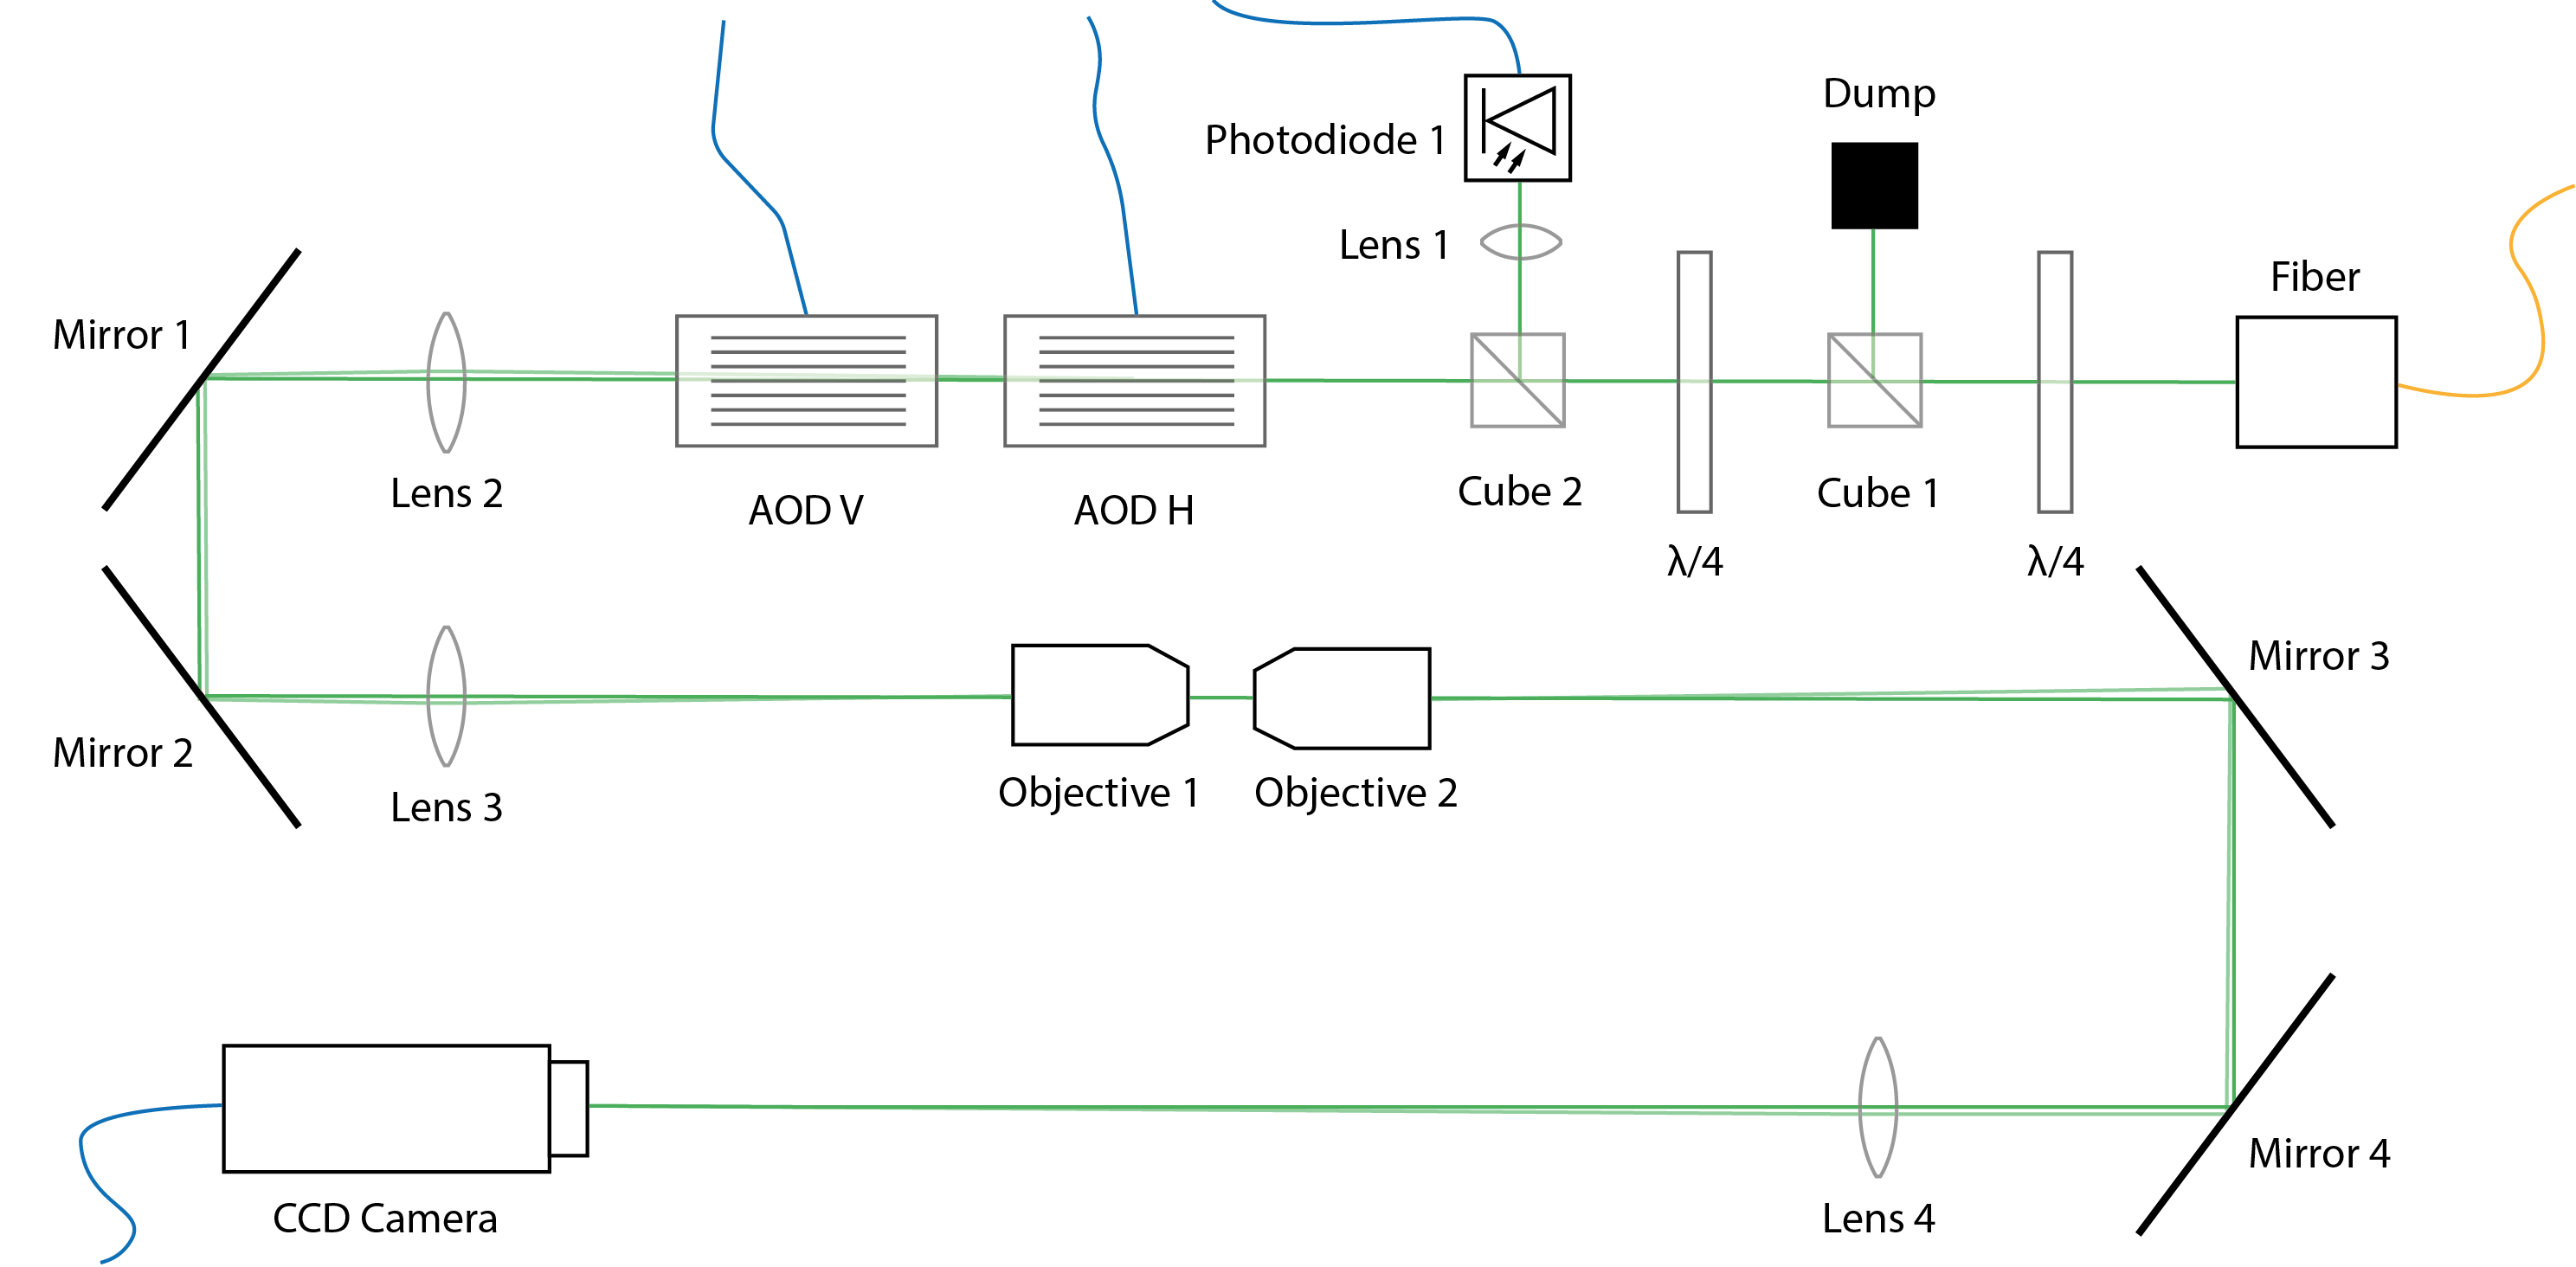
\includegraphics[width=\textwidth]{\mediadir{setup/intensity-profile.png}}
  \captionsetup{width=.8\textwidth}
  \caption{The beam is focused onto the \gls{ccd} sensor of the camera. The
    \gls{aod} are configured at \SI{100}{\mega\hertz} center frequency.
  }
  \label{fig:intensity_profile_setup}
\end{figure}

In \Cref{fig:intensity_profile_setup} we see the setup used to measure the
beam profile. The \gls{aod} are configured at \SI{100}{\mega\hertz} center
frequency. The distance between Lens 4 and the \gls{ccd} sensor is chosen
such that the the beam head is focused.

\subsection{Result}

In \Cref{fig:intensity_profile_2d} we can see an enlarged image patch of the
complete image caputre taken with the \gls{ccd} camera. We can see a strong
illuminated circular spot in the center of the iamge with an area of about
\SI{2.5}{\milli\meter}. The intensity inside the spot seems homogeneous,
however this is caused because the pixels are saturated in this area.
We could reduce the intensity or apply an optical filter to the camera to
resolve the intensity gradient inside the spot, but only at the cost of
the intensity distribution around the spot. Around the circular spot we can
see a diffraction ring. The diffraction ring is well described in
\cite{Hertlein2017} and originates from the finite aperture of the objectives.

\begin{figure}[ht]
  \centering
  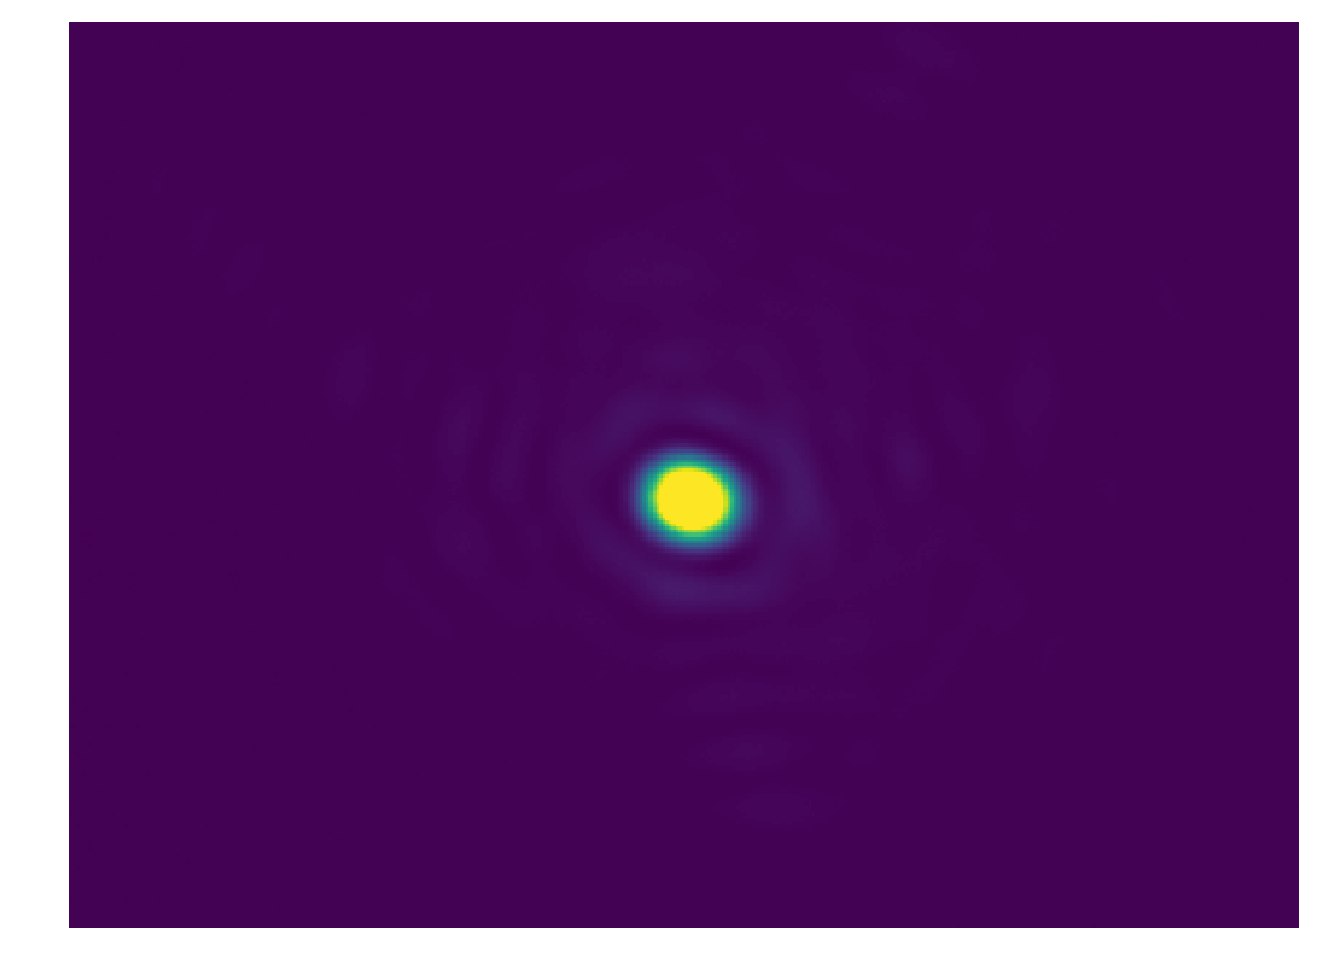
\includegraphics[width=.5\textwidth]{\figuredir{intensity/profile/profile2d.pdf}}
  \caption{Image detail from the captured beam with the \gls{ccd} camera.}
  \label{fig:intensity_profile_2d}
\end{figure}

Altough \Cref{fig:intensity_profile_2d} gives us a good overview of the
spatial beam profile it is difficult to see deviations from an ideal
gaussian curve in this representation. Henceforth we performed two
perpendicular cuts and visualized the one dimensional spatial beam
distribution in \Cref{fig:intensity_profile_1d}.

\begin{figure}[ht]
  \centering
  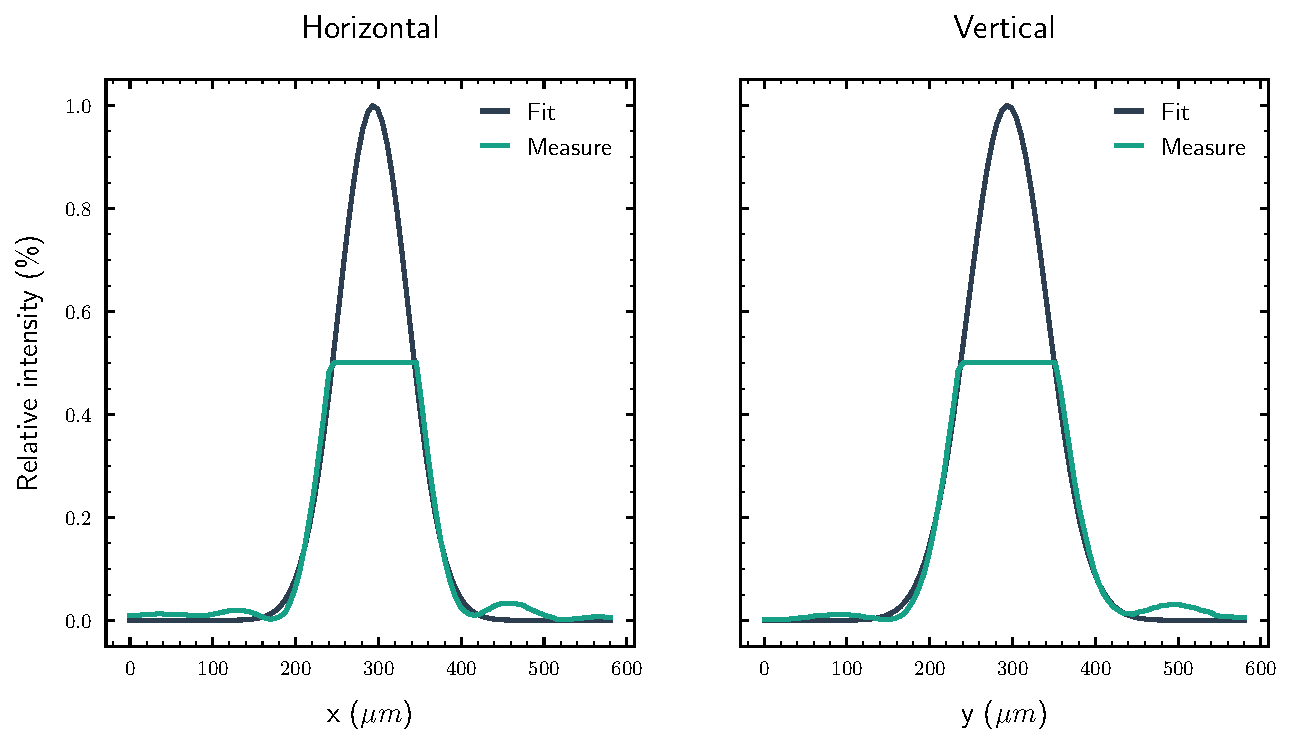
\includegraphics[width=\textwidth]{\figuredir{intensity/profile/profile1d.pdf}}
  \captionsetup{width=.8\textwidth}
  \caption{One dimensional perpendicular cut of the two dimensional beam
    distribution from the two dimensional beam profile in
    \cref{fig:intensity_profile_2d} with fitted gaussian curve.}
  \label{fig:intensity_profile_1d}
\end{figure}

In \Cref{fig:intensity_profile_1d} we can clearly observe the effects of
saturation around the center and how we would expect the intensity to be
if we could experimentally resolve it in the Gaussian fit. In contrast to the
ideal Gaussian profile we again observe contributions to the Airy disc around
the otherwise Gaussian profile causes by the finite aperture. Further we can
now clearly observe assymmetry from the intensity contributions around the
Gaussian which means that our alignment is not perfect.

\subsection{Summary}

We can confirm the results reported in \cite{Hertlein2017} that the spatial
beam profile equals a two dimensional Gaussian combined with a diffraction
ring caused from the finite aperture of the objectives. Further we observe
slight assymmetries in the diffraction ring suggesting inperfect alignment.

Though assymetries in the spatial beam profile are present, we do not see any
further complications as the intensity measurements with the photodiode will
cover the complete beam profile.
